\section{\SYSTEM{}: Combining Control and Learning}
\label{sec:framework}
A mobile device or embedded system runs a streaming application on a
heterogeneous processor.  We assume no prior knowledge of this
streaming application, but we do have prior knowledge of other
applications.  Our goal is to quickly build a model of the new
application and then control its resource usage such that it meets a
desired performance target with minimal energy.
\PUNT{
\begin{figure}
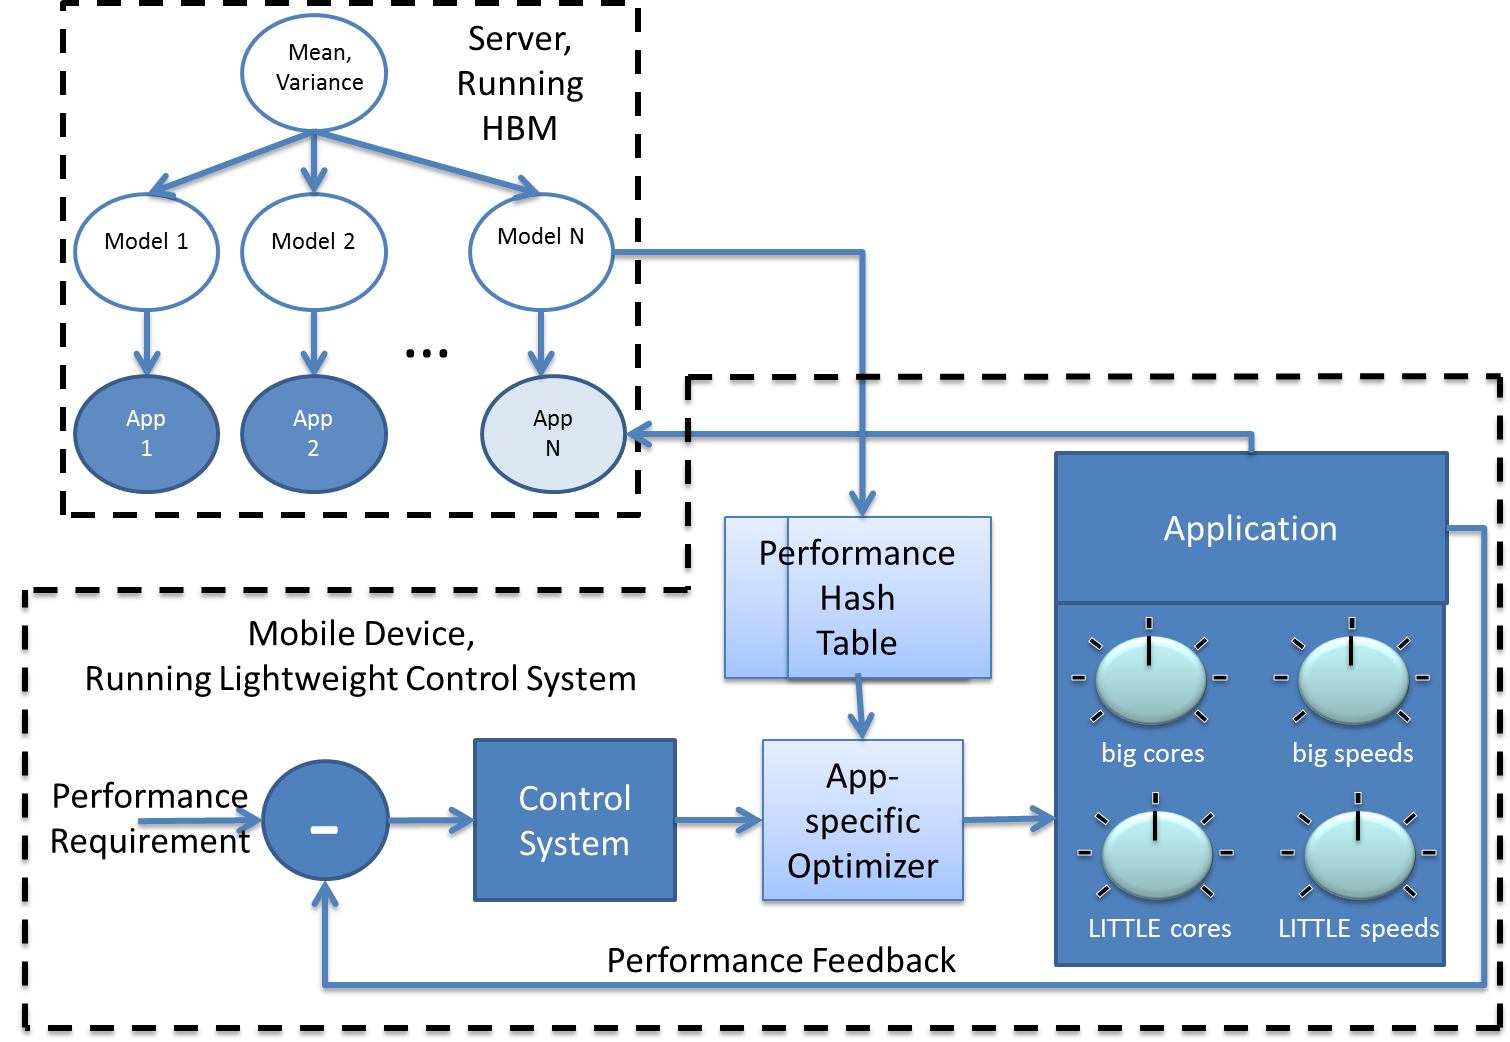
\includegraphics[width=\columnwidth]{figures/ControlLearning.png}
\caption{Overview of \SYSTEM{}.} 
\label{fig:overview}
\end{figure}
}

\figref{fig:overview} shows \SYSTEM{}'s approach to this problem.  On
the local device, a generalized control system (GCS) allocates
resources to the new application to meet its specified performance
goal with minimal energy.  The GCS starts with a generic resource
model, and as it selects configurations it records performance and
power in each configuration.  After recording a small number of values
(typically less than 10\% of the total configuration space).  These
recorded values are sent to a remote server which runs a hierarchical
Bayesian model (HBM).  The HBM estimates the application's performance
and power in all other configurations and extracts those
configurations that are Pareto-optimal in the performance/power
tradeoff space.  These configurations are packaged in a special data
structure -- the performance hash table (PHT) -- and sent to the GCS.
Using the PHT, the GCS selects an energy minimal resource
configuration in constant time ($O(1)$).  In addition to the PHT, the
server sends back the model's variance.  The GCS uses this variance to
customize control to the model's uncertainty, allowing guaranteed
convergence to the performance goal despite the fact that the system
starts with no prior knowledge of the streaming application.

The remainder of this section details \SYSTEM{}.  We begin by
describing a typical control design for a computer system and
illustrate how it fails to generalize.  We then describe \SYSTEM{}'s
generalized control system.  Next we discuss how \SYSTEM{} turns the
generalized control signal into specific resource configurations using
a model.  We then describe how to use a hierarchical Bayesian model to
estimate resource performance and power tradeoffs.  We then describe
the performance hash table that encodes the learned model. We conclude
with some brief analysis of the approach, with detailed analysis
provided in an appendix.


\section{Traditional Control Design for Computing Systems}
A controller has a performance goal (corresponding to a
quality-of-service or real-time constraint) and adjusts system resource
usage to see that the goal is met. Following is the general formulation for a controller, where the response is assumed to be linearly related to the effect.
\begin{equation}
  effect(t) = \alpha \cdot response(t-1) + \delta \label{eqn:clock}
\end{equation}
In a simple example, a control
system might adjust processor frequency to ensure that a performance
goal is met \cite{lefurgy}.  Even better, an optimal controller would
use the minimal clockspeed to meet the performance requirement.


To turn clockspeed into performance a controller needs a model
relating these two values.  Directly mapping clockspeed to performance
is difficult -- a hypothetical model might account for instruction
mixes, memory hierarchy, memory latency, synchronization overheads,
etc.  Building such a model is tedious and error-prone process and
that is before we address system dynamics (\eg applications
transitioning from memory to compute bound).  Instead, control systems
use relatively simple difference models\footnote{Continuous time
  systems would use differential equations, but as time in computers
  is inherently discretized we restrict ourselves to discussion of
  difference equations which are appropriate for discrete time
  systems.}. 

%example difference model -- built into the controller
Continuing the example of controlling performance with clockspeed, a
simple model appropriate for control would be to assume that the
performance is a linear function of the clockspeed:
\begin{equation}
  perf(t) = \alpha \cdot clock(t-1) + \delta \label{eqn:clock}
\end{equation}
Here, the observed performance $perf(t)$ is predicted as some constant
$alpha$ times the clockspeed applied at the previous time step,
$clock(t-1)$, plus some noise, $\delta$ drawn from a Gaussian
distribution.  This simple linear difference model ignores low-level
details like instruction mix, and instead uses feedback, predicting
behavior of the next time step as a function of the previous time
step.  Using the relationship of \eqnref{clock}, we can synthesize a
simple controller that is provably convergent to the desired
performance:
\begin{eqnarray}
  error(t) &=& goal - perf(t) \label{eqn:clock-error} \\
  clock(t) &=& clock(t-1) - \frac{error(t)}{k}
  \label{eqn:clock-control}
\end{eqnarray}


% Can we make the model a tunable parameter?
The controller of \eqnref{clock-control} provides formal guarantees
that it will converge to the desired performance ($goal$ in
\eqnref{clock-error}) and it bounds the time taken to converge.  All
these guarantees, however, are predicated on the accuracy of the
model; \ie on the value $alpha$ in this simple example.  This value is
highly dependent on the particular application under control.  More
complicated examples that control multiple resources are relatively
straightforward extensions of the example shown here that use matrix
equations instead of the scalar equations presented here
\cite{METE,others}.  Either way, the control system is highly
dependent on the value of $alpha$ -- we could set $alpha$ to be
application specific, but that controller will fail on some
applications.  If we choose a value of $alpha$ such that performance still
converges to the goal for all applications it will be very slow,
meaning that the controller will take many time steps to react to some
dynamic events.  It would clearly be beneficial to tune the control
models to individual applications.

\section{Generalized Control Design}
We would like to use control and learning to solve the problem of
meeting an application's performance requirements while minimizing
energy consumption.  The difficulty is that classical control
formulations like the example above integrate the models directly into
the controller; \ie the application-dependent relationship between
performance and resource usage is directly used in the control
equations.  We propose to address this problem using the classic
computer science trick of adding a layer of indirection.  This idea is
illustrated in \figref{overview}.  Instead of directly controlling
resources using an application-dependent model, we will control
\emph{speedup} and pass that speedup value to a separate module that
translates speedup into a desired resource configuration using the
learned models.  In this section, we first describe our formulation
for controlling speedup and then describe the translator that converts
that speedup into resource allocations.

\subsubsection{Controlling Speedup}
Analogous to \eqnref{clock} we write a simple difference model
relating speedup to performance:
\begin{equation}
  perf(t) = \alpha \cdot speedup(t-1) + \delta \label{eqn:speedup}
\end{equation}
where $b$ is the \emph{base speed} of the application, here defined as
the speed when all resources are available.  While $b$ is application
specific, it is easy to measure online, by simply allocating all
resources. Such a configuration should not violate any performance
constraints (although it is unlikely to be energy efficient) so it is
safe to take this measurement without risk of violating performance
constraints.

With this model, the control law is simply:
\begin{eqnarray}
  error(t) &=& goal - perf(t) \label{eqn:speedup-error} \\
  speedup(t) &=& speedup(t-1) - \frac{error(t)}{\alpha}
  \label{eqn:speedup-control}
\end{eqnarray}
which states that the speedup to apply at time $t$ is a function of
the previous speedup, the error at time $t$ and the base speed $\alpha$.
This is a very simple \emph{deadbeat} \TODO{need to add a pole -- so
  it will no longer be a deadbeat controller} controller that provides
all the standard control theoretic formal guarantees.  

By measuring
base speed online while the application runs, we can tune the control
to a specific application.  We note that using this definition of base
speed, most speedups will be less than one.  Another modification to \eqref{eqn:speedup-control} which gives a more general formulation,
\begin{equation}
speedup(t) = speedup(t-1) - \frac{1 - p}{\alpha}.error(t)
\end{equation}
This equation represents a less aggressive approach with a damping factor $1-p$, known as $pole$, to control the step-size taken to minimize the error term. The damping factor or the $pole$ guards the system from additional noise in the response. Additional details on the $pole$ and our new results connecting the value of pole with estimation error in the learning model are discussed in Section \secref{}.

\TODO{ Note sure}In addition to making
base speed easier to measure, this has the nice property of bounding
the learner's output, making for more robust learning \TODO{Nikita,
  what am I trying to say here? Or should we just put a forward
  reference because the next section benefits from a max speedup of 1}
Of course, we still have the challenging problem of converting an
abstract speedup into an actual resource allocation.


\section{Allocating Resources with a General Control Signal}
We need to map the speedup produced by \eqnref{speedup-control} into a
resource allocation.  On our target system, an ARM big.LITTLE
architecture, that specifically means mapping speedup into a number of
big cores, a number of small cores, and a speed for both (on our
system big and little cores can be clocked separately).

The primary challenge here is that the HBM produces a discrete
non-linear function of resource usage into speedup and powerup, while
\eqnref{speedup-control} is a continuous linear function.  We bridge
this divide by assigning time to resource allocations such that the
average speedup over a control interval is that produced by
\eqnref{speedup-control}.

We call an assignment of time to resources a schedule.  Not
surprisingly, there are typically many schedules that meet a
particular performance requirement.  We would like to find a minimal
energy schedule. Given a time interval $T$, a workload $W$ to
complete in that interval, and a set of $C$ configurations, we
formalize this problem as:
\begin{eqnarray}
  \minimize && \sum_{c=0}^{C-1} \tau_c \cdot p_c \label{eqn:power} \\
  \st %&& \nonumber\\
  && \sum_{c=0}^{C-1} \tau_c \cdot s_c \cdot b =  W \label{eqn:work} \\
  && \sum_{c=0}^{C-1} \tau_c =  T \label{eqn:deadline} \\
  && 0 \le \tau_c \le T, \qquad \forall c \in \{0,\ldots,C-1\} \label{eqn:time}
\end{eqnarray}
where $p_c$ and $s_c$ are the estimated powerup and speedup of
configuration $c$ and $\tau_c$ is the amount of time to spend in
configuration $c$.  \eqnref{power} simply states that the objective is
to minimize energy (power times time).  \eqnref{work} states that the
work must be done, while \eqnref{deadline} requires the work to be
done on time.  \eqnref{time} simply avoids negative time.  


\section{Learning Power/Performance Tradeoffs}

\begin{figure*}

  \subfloat[]
  {
    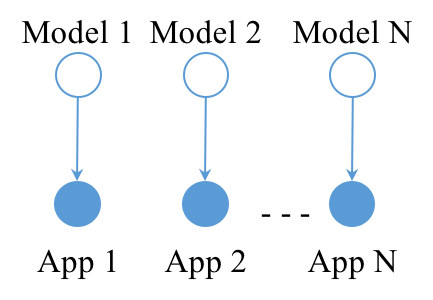
\includegraphics[width=.33\textwidth]{figures/Online.png}
    \label{fig:online}
  }
  \subfloat[]
  {
    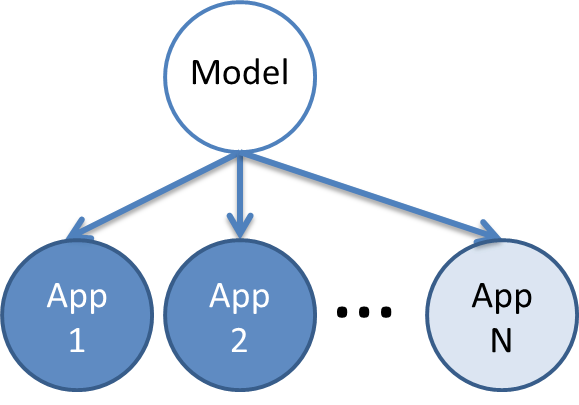
\includegraphics[width=.33\textwidth]{figures/Offline.png}
    \label{fig:offline}
  }
  \subfloat[]
  {
    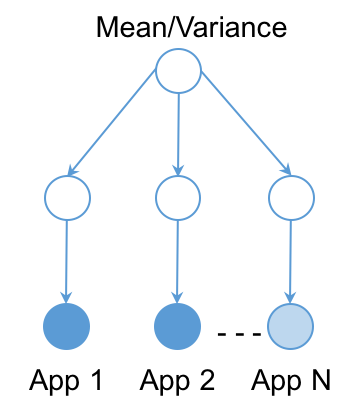
\includegraphics[width=.33\textwidth]{figures/HBM.png}
    \label{fig:HBM}
  }
  \caption{ Comparison of online (a) offline (b) and hierarchical
    Bayesian models (c).  The arrows represent dependences, circles
    are random variables, white circles are hidden variables that
    cannot be observed and must be learned, solid circles represent
    fully observed data, and shaded circles represent partially
    observed data.  The online model is concerned only with the
    current application (labeled N), the offline model combines all
    observations into one model, and the HBM builds per-application
    models, but makes them conditionally dependent on one another so
    that prior observations can be used to increase the accuracy of
    the model built for application N.}
\label{fig:learning-models}
\end{figure*}

In general, all machine learning techniques take observations of some
phenomena and turn them into a model to predict future outcomes.  In
our specific case, we want to take observations about application's
performance and power given a resource allocation and predict how
future application's will perform or how different resource
allocations will affect the current application.  

In this work, we use a hierarchical Bayesian model (HBM) to turn
observations of applications' performance and power into predictions
about how other, unobserved resource allocations will alter that
performance and power.  We use a HBM because it provides a
statistically sound framework for learning across applications and
devices.  The HBM is also well suited to learning the complicated
tradeoff spaces that arise from heterogeneity in modern mobile
processors.

When selecting a learning framework we must find a tradeoff between
the specific and the general; \ie between frameworks that build
application-specific models and frameworks that combine observations
across applications.  For example, the key to energy efficiency on
heterogeneous mobile systems is knowing when to make use of the
smaller, low-power cores \cite{}.  An application-specific model will
capture that precisely, but may require many observations before
producing the correct model.  A more general model will capture the
trend, \eg when most applications should transition, but this general
model might miss the key inflection point for some applications.  We
refer to application-specific models as \emph{online} because they
build models for the current application and do not incorporate
knowledge of other applications.  We refer to general models as
\emph{offline} as they use prior observations of other applications to
predict the behavior of a new application.  

The HBM provides a good balance between the online and offline
approaches.  The key differences between these three approaches are
illustrated in \figref{learning-models}. In this figure, circles
represent random variables, directed edges show conditionally
dependent relationships, and shading represents observability.  A dark
circle means we have seen all the data, a shaded circle means we have
some partial observations, and the white circle means that the
variable is unobservable.  The models we are trying to learn
are unobservable.  A strictly online approach will handle each new
application completely separately and ignore observations of previous
applications.  This approach never risks contaminating a model with
unrelated observations, but it may take many observations of the
current application to converge because it starts with no prior
knowledge. The offline approach uses all observations from prior
applications and will therefore converge very quickly; however, it is
overly general and cannot learn features specific to a single
application.

The HBM (illustrated in \figref{HBM}) is a good compromise.  Each
application has its own model, allowing specificity, but these models
are conditionally dependent on some underlying probability
distribution with a hidden mean and co-variance matrix.  In practice,
the HBM will estimate a model for a new application using a small
number of observations and combining those observations with the large
number of observations previously made of similar applications.
Rather than over-generalizing, the HBM will use only similar
applications to learn models.  In addition, the HBM's accuracy
increases as more applications are observed because more different
types of behavior are represented in the pool of prior knowledge.  Of
course, the computational complexity of learning also increases with
increasing applications, but this is why we offload the learning to a
remote server.

To provide intuition we offer a simple example.  Suppose we have
observed many prior applications, all of which are either completely
compute-bound or completely memory-bound, and we have an equal number
of both.  The only resource we can allocate is clockspeed, which will
increase the performance of compute-bound applications, but not
memory-bound ones.  When we need to work with a new application, we
need to estimate its response to clockspeed.  The online model will
not use prior knowledge, but will observe many different clock speeds
for the new application, leading to high overhead.  The offline model
will predict the mean response of prior applications, meaning it will
over-allocate speed to memory-bound applications and under-allocate to
compute-bound ones.  The HBM will take a small number of observations
and then the prediction will combine those with prior knowledge: if
the new observations show that clockspeed has no effect on performance
the HBM will use only the prior memory bound applications to build its
model, otherwise, it will use the compute-bound applications.  In
practice, the HBM can learn much more complicated tradeoffs by
combining observations of the new application with prior knowledge of
different types of behavior.

\section{Encoding Learned Models}


\TODO{This needs to be brief, and we can put any details in an
  appendix.}
  While most linear programming problems would be inefficient to solve
repeatedly on a mobile device, the one in \eqnrref{power}{time} has a
constant time ($O(1)$ solution.

Kim et al. analyzed heuristic solutions to the problem of minimizing
energy while meeting a performance constraint \cite{kim-cpsna}.  They
observed that there must be an optimal solution with the following
properties:
\begin{itemize}
\item At most two of $\tau_c$ are non-zero, meaning that at most two
  configurations will be used in any time interval.
\item If you chart the configurations in the power and performance
  tradeoff space (\TODO{add figure}) the two configurations with
  non-zero $\tau_c$ lie on the lower convex hull of the power
  performance tradeoff space.
\end{itemize}
We use these two facts to construct a constant time algorithm for
finding the optimal solution online.  


\begin{figure}
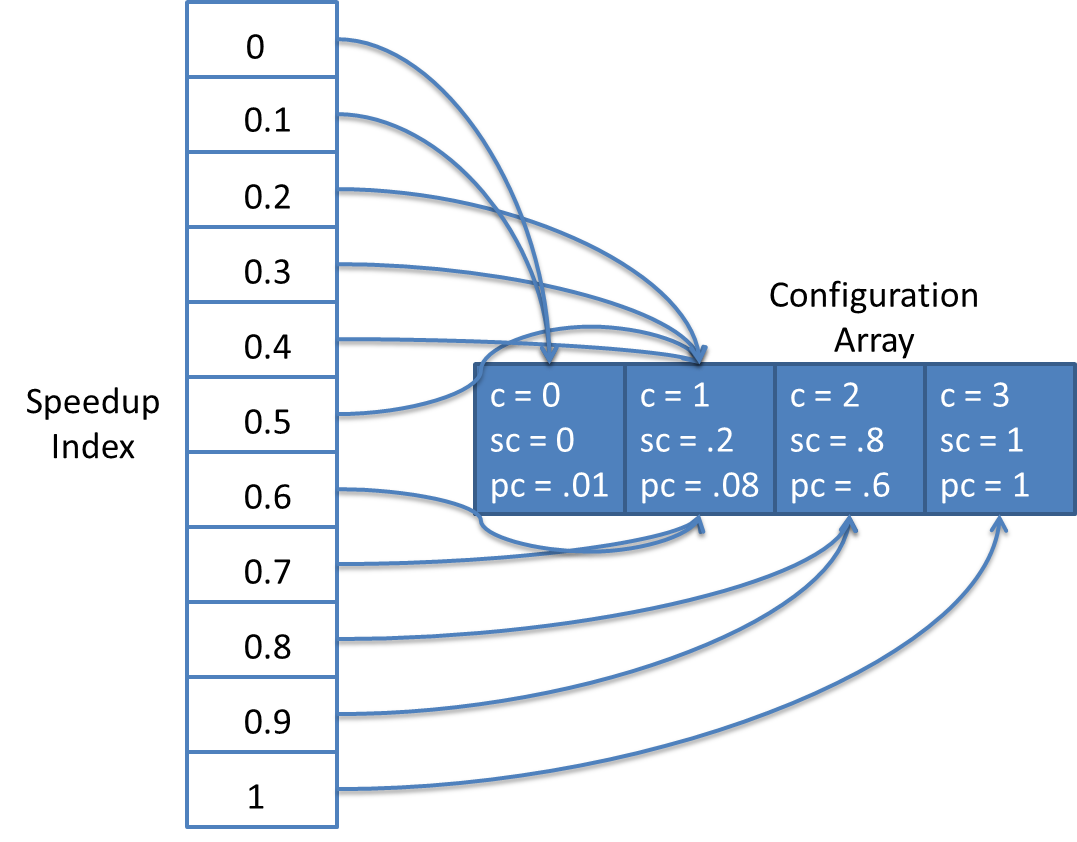
\includegraphics[width=\columnwidth]{figures/SpeedupHashTable.png}
\caption{Data structure to efficiently convert required speedup into a
  configuration.}
  \label{fig:pht}
\end{figure}



We create a \emph{performance hash table} (PHT).  The PHT will only
contain points on the lower convex hull of the power/performance
tradeoff space.  The PHT is illustrated in \figref{pht}.  It consists
of two arrays, the first is an array of pointers that point into the
second array, which stores the configurations on the convex hull
sorted by speedup.  Recall that speedups are computed relative to the
base speed which uses all resources.  We therefore know the largest
speedup is 1, so we need only concern ourselves with speedups less
than 1.  The first table, of pointers has a \emph{resolution}
indicating how many decimal points of precision it captures.  The
example in \figref{pht} has a resolution of .1.  Each pointer in the
first table points to the configuration in the second array that has
the largest speedup less than or equal to the index.

To use the table, the translator receives a speedup $s(t)$ from the
controller.  It needs to convert this into two configurations referred
to as $hi$ and $lo$.  To find the $hi$ configuration, the translator
clamps the desired speedup to the largest index lower than $s(t)$ and
then walks forward until it finds the first configuration with a
speedup higher than $s(t)$.  This configuration is $hi$.  To find the
$lo$ configuration, the translator clamps the desired speedup to the
smallest index higher than $s(t)$ and then walks backwards until it
finds the configuration with the largest speedup less than $s(t)$.

For example, consider the PHT in \figref{pht} and a translator trying
to meet a speedup $s(t) = .65$.  To find $hi$, the translator indexes
at .6 and walks up to find $c=2$ with $s_c=.8$, setting $hi = 2$.  To
find $lo$, the translator indexes the table at .7 and walks backward
to find $c=1$ with $s_c=.2$, setting $lo = 1$.

Finally, the translator sets $\tau_{hi}$ and $\tau_{lo}$ by solving the
following set of equations:
\begin{eqnarray}
  \tau &=& \tau_{hi} + \tau_{lo}    \label{eqn:s1} \\
  s(t) &=& s_{hi} \cdot \tau_{hi} + s_{lo} \cdot \tau_{lo} \label{eqn:s2} \\
\end{eqnarray}
In these equations, $s(t)$ is the speedup requested by the translator
and $s_c$ are speedups estimated by the learner. 

By solving \eqnsref{s1}{s2}, the translator has turned the speedup
requested by the controller into a schedule of resource allocations
using the models provided by the HBM.  Provided that the resolution is
large enough to get a good spread of configurations to indices, the
translator will always index the configuration array at most one entry
from where it needs to be.  Thus, the entire translation process runs
in constant time -- assuming that the learner is responsible for
building the PHT once before passing it on to the translator.  This
efficiency comes at a cost of memory usage -- many of the entries in
the speedup index table will point to redundant locations in the
configuration array.  We think that this is a reasonable tradeoff to
make in practice as the code that runs on the mobile device must be
fast or we risk wasting energy while trying to save energy.  In
practice, we recommend a table of size 100 which provides a sufficient
resolution and is not too wasteful of space.

\section{Analysis}
\subsection{Algorithmic Analysis}

\subsubsection{Control System Complexity}

\subsubsection{Learning System Complexity}

\subsection{Control Theoretic Formal Guarantees}
As we discussed in section \secref{}, a \emph{pole} acts as a damper in the control system equation \eqref{}. In this section, We would connect the concept of pole with the estimation procedure and obtain more sophisticated control system equations which take the estimation error into account.
The pole of a control system equation can be thought of as inversely proportional to "step-size" in gradient descent procedures. \TODO{more explanation}% When the system is deterministic, usually pole is chosen to be 0 since it leads to fastest convergence. But when the system

Suppose we allow the following multiplicative error in $response(t)$ or in our particular case $speedup(t)$, $\frac{speedup(t)}{\hat{speedup(t)}} \leq \Delta$. According to \cite{}, the value of pole $p$ can vary as much as, $\max(0,1-\frac{2}{\Delta}) \leq p \leq 1$, where $\Delta$ is the multiplicative error in the control equation. Using the lowest value of pole would offer the fastest convergence. We prove the following guarantees for the value of $\Delta$,

\begin{equation}
\Delta = 
\end{equation}

